\documentclass{beamer}
\usepackage[utf8]{inputenc}

\usepackage{hyperref}

\usepackage{graphicx}
\usepackage{float}
\usepackage{wrapfig}
\usepackage{algorithm}
\usepackage{algpseudocode}

\usepackage[style=numeric,maxnames=2]{biblatex}
\addbibresource{references.bib}

\setbeamertemplate{bibliography item}[text]

\DeclareBibliographyAlias{article}{std}
\DeclareBibliographyAlias{book}{std}
\DeclareBibliographyAlias{booklet}{std}
\DeclareBibliographyAlias{collection}{std}
\DeclareBibliographyAlias{inbook}{std}
\DeclareBibliographyAlias{incollection}{std}
\DeclareBibliographyAlias{inproceedings}{std}
\DeclareBibliographyAlias{manual}{std}
\DeclareBibliographyAlias{misc}{std}
\DeclareBibliographyAlias{online}{std}
\DeclareBibliographyAlias{patent}{std}
\DeclareBibliographyAlias{periodical}{std}
\DeclareBibliographyAlias{proceedings}{std}
\DeclareBibliographyAlias{report}{std}
\DeclareBibliographyAlias{thesis}{std}
\DeclareBibliographyAlias{unpublished}{std}
\DeclareBibliographyAlias{*}{std}

\DeclareBibliographyDriver{std}{%
  \usebibmacro{bibindex}%
  \usebibmacro{begentry}%
  \usebibmacro{author/editor+others/translator+others}%
  \setunit{\labelnamepunct}\newblock
  \usebibmacro{title}%
  \newunit\newblock
  \usebibmacro{date}%
  \newunit\newblock
  \usebibmacro{finentry}}

\usetheme{Madrid}
\usecolortheme{default}

\usepackage{shortcuts}

%------------------------------------------------------------
%Information to be included in the title page:
\title[Laplacian Score]{Laplacian Score for Feature Selection}

\subtitle{
    Xiafei He, Deng Cai, Partha Niyogi, 2005
}

\author{Jérémie Dentan and Gonzague de Carpentier \\ Professors: Laurent Oudre and Charles Truong}

\date{March 2023}
%------------------------------------------------------------

\begin{document}

\frame{\titlepage}

% Outline frame
\begin{frame}{Outline}
    \tableofcontents
\end{frame}

% Current section
\AtBeginSection[ ]
{
\begin{frame}{Outline}
    \tableofcontents[currentsection]
\end{frame}
}

\section{Introduction}
%------------------------------------------------------------
\begin{frame}
\frametitle{Introduction: Feature selection}

Paper under review: \textit{Laplacian Score for Feature Selection} \cite{he_laplacian_2005}.

\medskip

\begin{itemize}
    \item Why do we want to select features? \cite{guyon_introduction_2003}
    \begin{itemize}
        \item Better predictive performances
        \item Computational efficiency
        \item Need to measure fewer features
        \item Interpretability
    \end{itemize}
    
    \item What kind of method exist for that?
    \begin{itemize}
        \item \textbf{Wrapper methods}: Feature selection wrapped around task learning.
        \item \textbf{Filter methods}: Feature selection prior to task.
        \begin{itemize}
            \item Supervised: use labels
            \item Unsupervised: without labels
        \end{itemize}
    \end{itemize}
\end{itemize}

\medskip

The \textbf{Laplacian Score} is an unsupervised filter method.

Idea: Preserve the structure of the nearest neighbors graph.

\end{frame}
%------------------------------------------------------------

\section{Method}
%------------------------------------------------------------
\begin{frame}
\frametitle{Laplacian Score}

\begin{enumerate}
    \item \textbf{Compute the nearest neighbor graph $G$:} 
    $$G_{i,j} := \begin{cases} 
        1 & \text{if $x_i$ is among the $k$ nearest neighbors of $x_j$ or reciprocally} \\
        0 & \text{otherwise}
    \end{cases}$$
    \item \textbf{Compute the weighted adjacency matrix $S$:}
    $$S := G \odot \exp\left(- \frac 1 {\sigma^2} M^2 \right) \in \RR^{m\times m}$$
    \item \textbf{Compute the degree matrix $D$:}
    $
        D := \diag(S\one) \in \RR^{m\times m}
    $
    \item \textbf{Compute the centered features $\Tilde{f}$:} 
    $
        \Tilde{f}_r = f_r - \frac {f_r^T D \one} {\one^T D \one} \one
    $
    \item \textbf{Compute the laplacian scores $L_r$:} 
    $$L_r := \frac{\Tilde{f}_r^T L \Tilde{f}_r}{\Tilde{f}_r^T D \Tilde{f}_r} \in [0, 1] \ \ \ \ \ L := D - S$$
    \item \textbf{Select the features} having the highest Laplacian scores.
\end{enumerate}

\end{frame}
%------------------------------------------------------------
\begin{frame}
\frametitle{Our experiments}

What will we do?
\begin{itemize}
    \item Evaluate the impact of the \textbf{hyperparameters} $\sigma$ and $k$
    \item Evaluate the impact of using \textbf{DTW} or the euclidian distance
    \item \textbf{Compare} the method to classical feature selection methods: (1) a simple variance threshold (unsupervized) and (2) filtering on the ANOVA score \cite{scheffe_analysis_1999} (supersized).
\end{itemize}

\medskip

How do we measure the performance?
\begin{itemize}
    \item \texttt{sklearn}'s SVC with default parameters
    \item Measure the accuracy for binary classification based on the same set of features
\end{itemize}

\end{frame}
%------------------------------------------------------------

\section{Data}
%------------------------------------------------------------
\begin{frame}
\frametitle{Data}

Three datasets from \href{https://timeseriesclassification.com}{\color{blue}{https://timeseriesclassification.com}}:

\begin{itemize}
    \item \textbf{Earthquakes} \cite{bagnall_earthquakes_nodate}: 
    \begin{itemize}
        \item Data: readings from Northern California Earthquake Data Center
        \item Labels: major earthquake event or not
    \end{itemize}
    \item \textbf{Wafer} \cite{olszewski_wafer_nodate}:
    \begin{itemize}
        \item Data: process control measurements during the processing of silicon wafers
        \item Labels: normal or abnormal
    \end{itemize}
    \item \textbf{WormsTwoClass} \cite{brown_wormtwoclass_nodate}:
    \begin{itemize}
        \item Data: projection of the motion of worms on a particular dimension, second-long intervals
        \item Labels: wild-type or mutant
    \end{itemize}
\end{itemize}

\end{frame}
%------------------------------------------------------------

%------------------------------------------------------------
\begin{frame}
\frametitle{Data visualization}

\begin{figure}
    \centering
    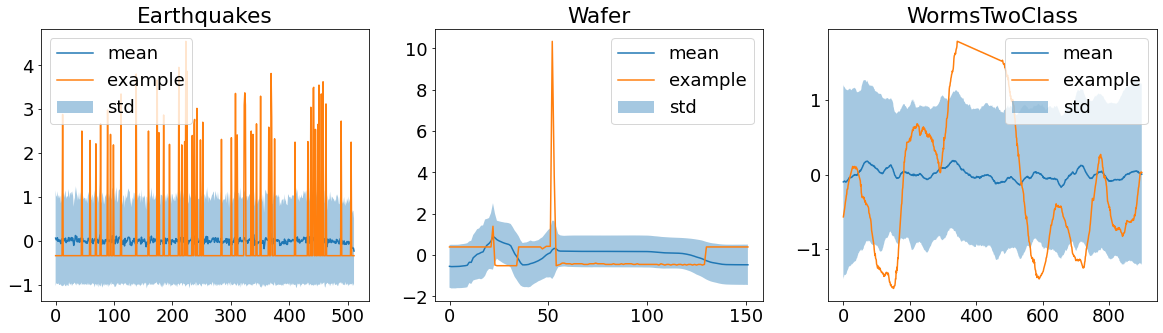
\includegraphics[width=0.9\textwidth, keepaspectratio=True]{figures/ds_visualization.png}
    \caption{Visualization of the three datasets. For each dataset, we plot the average time series, the standard deviation at each timestamp and an example sampled randomly from the dataset.}
    \label{fig:ds_visulization}
\end{figure}

\end{frame}
%------------------------------------------------------------

%------------------------------------------------------------
\begin{frame}
\frametitle{Autocovariance functions}

\begin{figure}
    \centering
    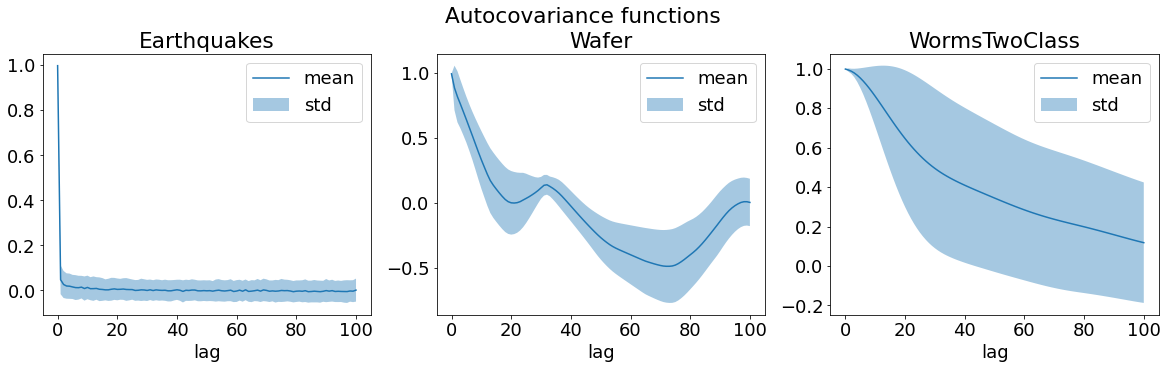
\includegraphics[width=0.9\textwidth, keepaspectratio=True]{figures/ds_acov.png}
    \caption{Average autocovariance functions for the three datasets.}
    \label{fig:ds_acov}
\end{figure}

\medskip
Then, we used TSFEL \cite{barandas_tsfel_2020} to extract the features.

\end{frame}
%------------------------------------------------------------

\section{Results}
%------------------------------------------------------------
\begin{frame}
\frametitle{Distribution of the Laplacian Scores}

3 regimes:
\begin{itemize}
    \item $\sigma$ small: $S \rightarrow 0$, scores concentrated around $0$
    \item Transition phase
    \item $\sigma$ huge: $S \rightarrow G$, so the scores also converge
\end{itemize}
\medskip
\begin{figure}
    \centering
    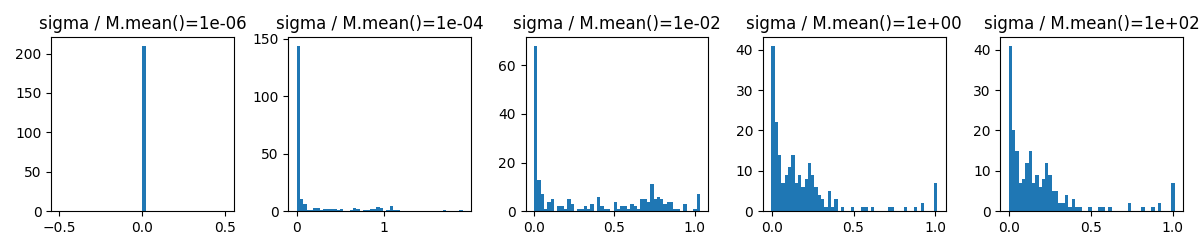
\includegraphics[width=\textwidth, keepaspectratio=True]{figures/laplacian_histograms.png}
    \caption{Histograms of the value of the Laplacian score for several values of $\sigma / \overline{M}$}
    \label{fig:sigma_histograms}
\end{figure}

\end{frame}
%------------------------------------------------------------

%------------------------------------------------------------
\begin{frame}
\frametitle{Influence of $\sigma$}

\begin{itemize}
    \item For some datasets, the task is either too simple or too difficult
    \item Good heuristic: take $\sigma$ quite small
\end{itemize}
\medskip
\begin{figure}
    \centering
    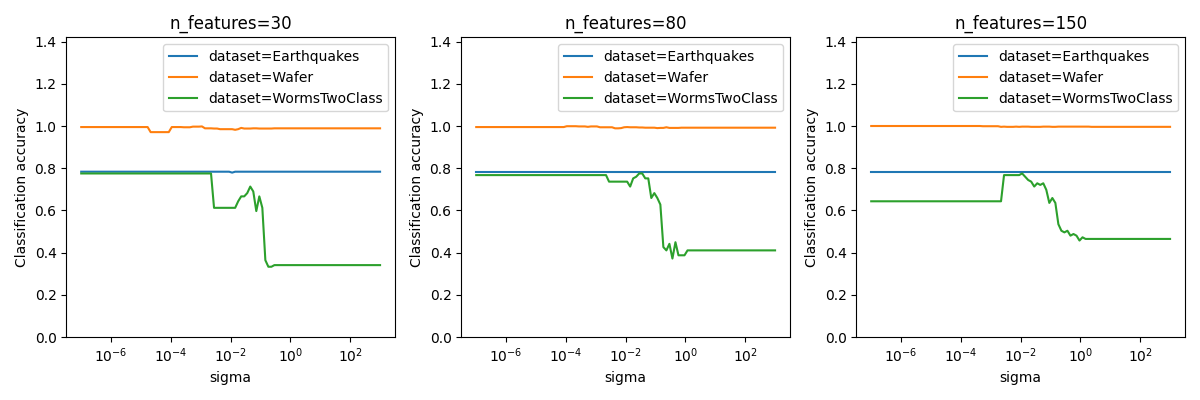
\includegraphics[width=0.95\textwidth]{figures/accuracy_vs_sigma.png}
    \caption{Evolution of the classification accuracy against the value of $\sigma$.}
    \label{fig:accuracy_vs_sigma}
\end{figure}

\end{frame}

%------------------------------------------------------------

%------------------------------------------------------------
\begin{frame}
\frametitle{Influence of the number of nearest neighbors}

\begin{figure}
    \centering
    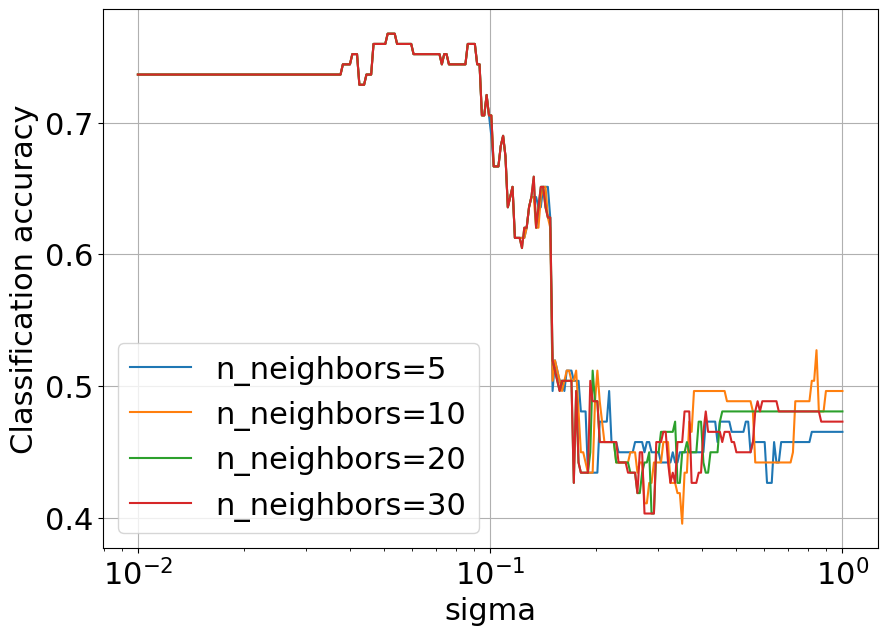
\includegraphics[width=0.6\textwidth]{figures/accuracy_vs_sigma_and_nnn.png}
    \caption{Evolution of the classification accuracy against the value of sigma.}
    \label{fig:accuracy_vs_n_features}
\end{figure}

$\Rightarrow$ Good heuristic: take $\sigma / \overline{M}$ small, around $10^{-4}$, and $k$ medium, of the order of ten.

\end{frame}
%------------------------------------------------------------

%------------------------------------------------------------
\begin{frame}
\frametitle{Comparison with other selection methods}

\begin{figure}
    \centering
    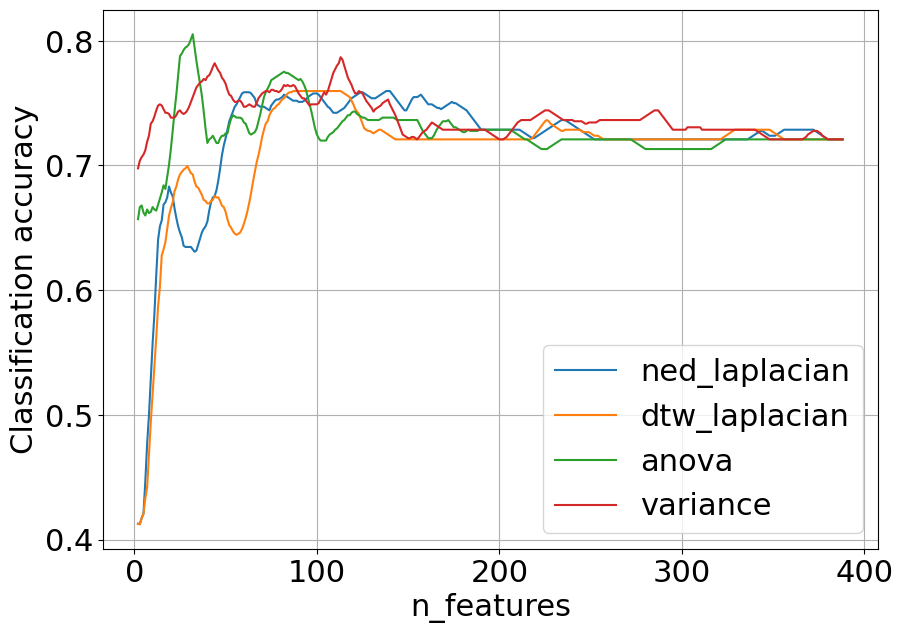
\includegraphics[width=0.5\textwidth]{figures/accuracy_vs_n_features.png}
    \caption{Evolution of the classification accuracy against the number of features.}
    \label{fig:accuracy_vs_n_features}
\end{figure}

\begin{itemize}
    \item Similar, but slightly lower performance
    \item DTW is not better than euclidian distances here
\end{itemize}

\medskip
\small{\textit{NED = Normalized Euclidian Distance}}


\end{frame}
%------------------------------------------------------------

%------------------------------------------------------------
\begin{frame}
\frametitle{Conclusion}

\begin{itemize}
    \item Advantage: unsupervised method
    \item Drawback: 2 hyperparameters to tune. Not very stable.
    \item Interesting method but perfomance on tested datasets and task is not overwhelming.
\end{itemize}

\end{frame}
%------------------------------------------------------------

%------------------------------------------------------------
\begin{frame}
\frametitle{References}
\nocite{he_laplacian_2005}
\printbibliography
\end{frame}
%------------------------------------------------------------

\end{document}

